\chapter{Preliminares}\label{ch:preliminares}

Este capítulo contiene dos partes muy importantes para entender la base teórica del trabajo. En la primera parte se dan definiciones generales sobre el álgebra lineal, las cuales son necesarias para la segunda parte en la que se introduce la mecánica cuántica en términos de matrices de densidad.
Al final se detallan algunos conceptos adicionales que resultan útiles más adelante.

\section{Álgebra Lineal}
El álgebra lineal es el estudio de espacios vectoriales y operaciones lineales sobre esos espacios. Para entender mecánica cuántica es necesario un conocimiento firme en álgebra lineal. En esta sección se definen algunos conceptos y notaciones que serán útiles más adelante, inspirados en los libros \cite{quantum_computer_science} y \cite{purification}.

\subsection{Vectores}

Los objetos elementales del álgebra lineal son los \emph{espacios vectoriales}. El espacio que más nos interesa es el de $\gen{C}^n$, el espacio de todas las $n$-tuplas de números complejos, $(z_1, \dots, z_n)$. Los elementos de este espacio son \emph{vectores}, con sus operaciones de adición y multiplicación por escalar habituales. Suelen representarse también cómo una matriz de $n \times 1$, es decir una columna de $n$ filas, en cuyo caso se denominan vector columna.
La notación estándar en mecánica cuántica de un vector en un espacio vectorial es la siguiente:
\[\ket{\phi}\]

$\phi$ es una etiqueta del vector y la notación $\ket{\cdot}$ es usada para indicar que el objeto es un vector columna. El objeto $\ket{\phi}$ es conocido también como \emph{ket}.

El espacio vectorial contiene también un elemento especial $\vec{0}$, el vector cero. El mismo cumple con la propiedad $\ket{v} + \vec{0} = \ket{v} \;\forall \ket{v}$. Es importante no confundir este vector con $\ket{0}$ el cual se reserva para significar algo completamente distinto (en la Sección~\ref{sub:postulados}).

\subsection{Bases e independencia lineal}
Un \emph{generador} es un conjunto de vectores $\ket{v_1}, \dots, \ket{v_n}$ de un espacio vectorial $V$ tales que cualquier vector $\ket{v}\in V$ puede ser escrito como una combinación lineal $\ket{v} = \sum_i a_i \ket{v_i}$ de los vectores del conjunto. 

\begin{ejemplo}
    Un generador de $\gen{C}^2$ es el conjunto:
\begin{equation*}
    \ket{v_1}= \begin{bmatrix}
        1\\0
    \end{bmatrix}; \ket{v_2} = \begin{bmatrix}
        0\\1
    \end{bmatrix}.
\end{equation*}
\end{ejemplo} 

Decimos que $\ket{v_1}$ y $\ket{v_2}$ generan el espacio vectorial $\gen{C}^2$. Otro ejemplo de generador para $\gen{C}^2$ es:
\begin{equation*}
    \ket{v_1}= \frac{1}{\sqrt{2}}\begin{bmatrix}
        1\\1
    \end{bmatrix}; \ket{v_2} = \frac{1}{\sqrt{2}}\begin{bmatrix}
        1\\-1
    \end{bmatrix},
\end{equation*}

puesto que cualquier vector $\ket{v}= (a_1, a_2)$ puede ser escrito como una combinación lineal de $\ket{v_1}$ y $\ket{v_2}$:

\begin{equation*}
    \ket{v}= \frac{a_1+a_2}{\sqrt{2}}\ket{v_1} +  \frac{a_1-a_2}{\sqrt{2}}\ket{v_2}.
\end{equation*}

\begin{definicion}
Un conjunto de vectores no nulos $\ket{v1}, \dots, \ket{v_n}$ es \emph{linealmente dependiente} si existe un conjunto de números complejos $a_1, \dots, a_n$ con $a_i\neq 0$ para al menos un valor de $i$, tal que $a_1\ket{v_1} + \dots + a_n\ket{v_n} = 0$.
\end{definicion}


Se dice que un conjunto de vectores es linealmente independiente si no es linealmente dependiente. Se puede demostrar que cualquier conjunto de vectores independientes que generan un espacio vectorial $V$ contiene la misma cantidad de elementos. Llamamos a tal conjunto una base de $V$. Además, tal base siempre existe. El número de elementos de la base se define como la dimensión de $V$. En este trabajo estamos interesados solamente en espacios vectoriales con dimensiones finitas.

\subsection{Operadores lineales}
Un operador lineal entre los espacios vectoriales $V$ y $W$ se define como una función $A: V \rightarrow W$ que es lineal en su entrada, es decir:

\begin{equation}\label{eq:op_lineal}
    A\left(\sum_i a_i\ket{v_i}\right) = \sum_i a_i A \left(\ket{v_i}\right).
\end{equation}

La forma más conveniente de entender los operadores lineales es en términos de sus representaciones matriciales. De hecho, el paradigma de los operadores lineales y las matrices resultan ser equivalentes. Para ver la conexión, es útil comprender primero que una matriz $A$ compleja de $m\times n$ con entradas $A_{ij}$ es, de hecho, un operador lineal que envía vectores en el espacio vectorial $\gen{C}^n$ al espacio vectorial $\gen{C}^m$, utilizando la multiplicación entre $A$ y vectores en $\gen{C}^n$. Con esta definición es fácil ver como $A$ cumple con la definición de operador lineal de la Ecuación~\ref{eq:op_lineal}.

Habiendo visto que las matrices pueden ser vistas como operadores lineales, ¿pueden los operadores lineales ser vistos como matrices? Suponga que $A: V \rightarrow W$ es un operador lineal entre los espacios vectoriales $V$ y $W$. Suponga que $\ket{v_1}, \dots, \ket{v_n}$ es una base de $V$ y $\ket{w_1}, \dots, \ket{w_m}$ es una base de $W$. Entonces por cada $j$ en el rango $1, \dots, m$ sabemos que $A\ket{v_j}\in W$, por lo que existe una descomposición en la base $\{w_i\}$. Es decir, existe una serie de números complejos $A_{1j}, \dots, A_{nj}$ tales que:

\[A\ket{v_j} = \sum_i A_{ij} \ket{w_i}.\]

La matriz cuyos valores son compuestos por los valores $A_{ij}$ se la conoce como la \emph{representación matricial} del operador $A$. Esta matriz es equivalente al operador $A$ y ambas abstracciones son intercambiables.

\subsection{Producto interno}

El productor interno es una función que toma dos vectores $\ket{v}$ y $\ket{w}$ de un espacio vectorial y devuelve un número complejo. La notación para esta operación en mecánica cuántica es $\braket{v|w}$.
Una función $\braket{\cdot|\cdot}$ de $V \times V \rightarrow \gen{C}$ es un producto interno  si satisface que:
\begin{enumerate}
    \item  Es lineal en su segundo argumento:
    \begin{equation}
        \braket{v|\sum_i \lambda_i \ket{w_i}} = \sum_i \lambda_i \braket{v|w_i}.
    \end{equation}
    \item $\braket{v|w} = \braket{w|v}^*$, donde $*$ denota el conjugado del número complejo.
    \item $\braket{v|w} \geq 0$, con la igualdad dándose si y solo si $\ket{v} = 0$.
\end{enumerate}

El productor interno utilizado para $\gen{C}^n$ se define como:

\begin{equation}\label{eq:inner_prod}
    \braket{\begin{bmatrix}y_1 \\ \vdots \\ y_n\end{bmatrix} | \begin{bmatrix}z_1 \\ \vdots \\ z_n\end{bmatrix}} = \sum_i y_i^* z_i = \begin{bmatrix}
y_1^* & \dots & y_n^*
\end{bmatrix} \begin{bmatrix}
    z_1 \\
    \vdots \\
    z_n
\end{bmatrix}.
\end{equation}

Donde el primer $*$ denota el transpuesto conjugado de la representación matricial del vector.

Llamamos como \emph{espacio prehilbertiano} a un espacio vectorial equipado con un producto interno.


\subsubsection{Notación Bra}
La notación $\bra{v}$ es usada para denotar el \emph{vector dual} de $\ket{v}$. El dual de un vector es un operador lineal que se define sobre un espacio prehilbertiano de la siguiente manera: $\bra{v}(\ket{w}) = \braket{v|w}$. En la Sección~\ref{sub:hilbert} se muestra que para el espacio $\gen{C}^n$, el vector dual es simplemente un vector fila.

\subsubsection{Vectores normalizados}


Los vectores $\ket{w}$ y $\ket{v}$ son ortogonales si su producto interno es cero. Por ejemplo, \(\ket{w}=\begin{bsmallmatrix}
    1 & 0
\end{bsmallmatrix}^*\) y \(\ket{v}=\begin{bsmallmatrix}
    0 & 1
\end{bsmallmatrix}^*\) son ortogonales con respecto al producto interno definido en \ref{eq:inner_prod}. Definimos la norma del vector $\ket{v}$ como
\begin{equation}
    \norma{\ket{v}} = \braket{v|v}.
\end{equation}


Un vector unitario es un vector $\ket{v}$ tal que $\norma{\ket{v}} = 1$. También decimos que $\ket{v}$ está normalizado si es unitario. Un conjunto de vectores $\ket{i}$ con índice $i$ es ortonormal si cada vector es unitario y son ortogonales entre sí, es decir, $\braket{i|j} = \delta_{ij}$, donde $i$ y $j$ pertenecen al conjunto y \(\delta_{ij} = \begin{cases}
1 \quad\text{si } i\neq j\\
0 \quad\text{si } i=j
\end{cases}\).
`
\begin{definicion}[Adjunto]
El adjunto de un operador $A$ se nota por $A^\dagger$ y se define como el operador transpuesto y conjugado de $A$. Es decir, si $\alpha_{ij}=\braket{u_i|A|u_j}$ son las componentes de $A$, las componentes de $A^\dagger$ son $\alpha^*_{ij} = \braket{u_j|A|u_i}^* = \braket{u_i|A^\dagger|u_j}$.
\end{definicion}

\begin{definicion}[Operador Hermitiano]
    Un operador $A$ cuyo adjunto es $A$ se lo llama operador \emph{Hermitiano}.
\end{definicion}

\begin{definicion}[Operador normal]
Un operador $A$ es normal si $AA^\dagger = A^\dagger A$. Claramente, un operador Hermitiano es también normal. 
\end{definicion}

\subsection{Espacio de Hilbert}\label{sub:hilbert}

La mecánica cuántica gira en torno a los \emph{espacios de Hilbert} porque son utilizados para describir el estado de los sistemas cuánticos. En el espacio dimensional finito y complejo con el que se trabaja en computación e información cuántica, un espacio prehilbertiano es automáticamente un espacio de Hilbert. Se prefiere el término espacio de Hilbert, pero basta con saber que si se trata de espacios prehilbertianos con infinitas dimensiones, el mismo debe satisfacer requerimientos adicionales para ser considerado espacio de Hilbert.



Con estas convenciones, al producto interno de un espacio de Hilbert se le puede asignar una conveniente representación matricial. Siendo $\ket{w} = \sum_i w_i\ket{i}$ y $\ket{v} = \sum_i v_i\ket{i}$ representaciones de dos vectores bajo una base ortonormal $\ket{i}$. Entonces, como $\braket{i|j} = \delta_{ij}$,

\begin{equation}
    \braket{v|w} = \sum_{ij} v_i^* w_j \delta_{ij}  = \sum_i v_i^* w_i.
\end{equation}

De esta manera el producto interno de dos vectores es igual al producto vectorial interno entre las dos representaciones matriciales de esos vectores, asumiendo que ambas representaciones son sobre la misma base ortonormal. También vemos como el vector dual $\bra{v}$ se puede representar como el vector fila donde sus componentes son el conjugado complejo de las componentes del vector columna de la representación de $\ket{v}$.

Una manera útil de representar operadores lineales es a través del producto interno, con un método conocido como representación del producto externo. Sea $\ket{v}$ un vector en un espacio prehilbertiano $V$ y $\ket{w}$ un vector en un espacio prehilbertiano $W$. Definimos $\ket{w}\bra{v}$ como el operador lineal de $V$ a $W$ cuya acción es definida por:
\begin{equation}
    (\ket{w}\bra{v}) (\ket{v'}) = \ket{w} \braket{v|v'} = \braket{v|v'} \ket{w}.
\end{equation}

Esta ecuación encaja maravillosamente en nuestras convenciones de notación, según la que la expresión $\ket{w}\braket{v|v'}$ podría tener dos significados: el resultado de operar $\ket{w}\bra{v}$ sobre $\ket{v'}$, o el resultado de multiplicar $\ket{w}$ por el número complejo $\braket{v|v'}$. ¡Nuestras definiciones fueron elegidas de manera que estás dos interpretaciones son equivalentes!



\subsection{Autovectores y autovalores}

Un \emph{autovector} de un operador lineal $A$ (dentro de un espacio vectorial) es un vector $\ket{v}$ no nulo tal que $A\ket{v}=\lambda \ket{v}$, donde $\lambda$ es un número complejo conocido como el autovalor de $A$ asociado a $\ket{v}$. Se asume que el lector está familiarizado con las propiedades elementales de los autovalores y autovectores, en particular, cómo obtenerlos vía la ecuación característica. La \emph{ecuación característica} se define como $c(\lambda) = \text{det} \| A - \lambda I\|$, donde $\text{det}$ es la función determinante de las matrices. Se puede demostrar que la función característica depende solo del operador $A$, y no de la representación matricial que tenga $A$. Las soluciones de la ecuación $c(\lambda) = 0$ son los autovalores del operador $A$. Por el teorema fundamental del álgebra, todo polinomio tiene por lo menos una raíz compleja, por lo que todo operador $A$ tiene por lo menos un autovalor, y su autovector correspondiente. El autoespacio correspondiente al autovalor $\lambda$ es el conjunto de vectores que tienen a $\lambda$ como su autovalor. %Es un subespacio del espacio vectorial sobre el cuál $A$ opera.

\begin{definicion}[Representación diagonal]
    Una \emph{representación diagonal} del operador $A$ en un espacio vectorial $V$ es una representación $A = \sum_i \lambda_i \ket{i}\bra{i}$, donde los vectores $\ket{i}$ forman una base ortonormal de autovalores para $A$, siendo $\lambda_i$ sus autovalores asociados. Un operador es \emph{diagonalizable} si tiene una representación diagonal.
\end{definicion}

\begin{definicion}[Operador positivo]
Un operador $A$ se dice \emph{positivo} si para todo
  vector $\ket\psi$, $\bra\psi A\ket\psi\geq 0$. Si $\bra\psi A\ket\psi >0$ para
  todo $\ket\psi\neq 0$, decimos que $A$ es \emph{definido positivo}.
\end{definicion}

\begin{teorema}[Descomposición espectral]
Todo operador normal $M$ en un espacio vectorial $V$ es diagonal con respecto a una base ortonormal de $V$. A su vez, todo operador diagonalizable es normal.
\end{teorema}
\begin{proof}
    Se encuentra demostrado por inducción en la dimensión de $V$ en la página 72 del libro \cite{purification}.
\end{proof}

\begin{teorema}[Descomposición del operador positivo]\label{teo:descomposicion}
Se puede demostrar que todo operador positivo es automáticamente Hermitiano y, por lo tanto, posee por la descomposición espectral una representación diagonal $\sum_i \lambda_i\ket{i}\bra{i}$. Además, sus autovalores son no negativos ($\lambda_i \in \mathbb{R}_0^+$).
\qed
\end{teorema}

\begin{definicion}[Operador unitario]
Un operador $A$ es unitario si $AA^\dagger = A^\dagger A = I$. Claramente, un operador unitario es también normal. 
\end{definicion}

\subsection{Producto tensorial}
El producto tensorial es una forma de combinar espacios vectoriales para formar espacios vectoriales más grandes. Esta construcción es fundamental para comprender la mecánica cuántica de sistemas compuestos.

Sean $V$ y $W$ dos espacios vectoriales con bases canónicas $B = \{b_i | i \in I\}$ y $C = \{c_j | j \in J\}$ respectivamente. El producto tensorial $V\otimes W$ de $V$ y $W$ es el espacio vectorial de base canónica \(\{b_i\otimes c_j |i\in
 I, j \in J \}\), donde $b_i \otimes c_j$ es el par ordenado formado por el vector $b_i$ y el vector $c_j$. La operación $\otimes$ se extiende a vectores de $V$ y $W$ bilinealmente:

\begin{equation}
(\sum_i \alpha_i b_i ) \otimes (\sum_j \beta_j c_j) = \sum_{ij} \alpha_i \beta_j (b_i \otimes c_j).
\end{equation}

\textit{Observación.} Notar que $V \times W \neq V\otimes W$. Por ejemplo, si $V = W = \gen{C}^2$, con base canónica $\{i,j\}$, entonces $V\times W$ contiene  a $i\otimes i$ y a $j\otimes j$, pero no a $i\otimes i+j\otimes j$, que no es producto de dos vectores de $\gen{C}^2$.

\begin{propiedades}[del producto tensorial] Sean $A, B, C, D$ operadores y $\ket{a}, \ket{b}, \ket{c}, \ket{d}$ vectores de un espacio de Hilbert.

  \begin{multicols}{2}
    \begin{enumerate}
    \item $(A\otimes B)(C\otimes D) = AC \otimes BD$, si $AC$ y $BD$ son multiplicaciones válidas.
    \item $\adj{(A\otimes B)} = \adj{A}\otimes\adj{B}$
    \item $\braket{\ket{a}\otimes \ket{b} | \ket{c} \otimes \ket{d}} = \braket{a|c}\braket{b|d}$ %https://physics.stackexchange.com/questions/129280/inner-products-containing-the-tensor-product-of-two-operators
    \item $(A\otimes B) (\ket{a} \otimes \ket{b}) = A\ket{a} \otimes B\ket{b}$ 
    \end{enumerate}
  \end{multicols}
    
\end{propiedades}

\section{Computación cuántica}
 
Si bien la computación cuántica es un campo muy interesante y en rápida evolución, no entraremos en gran detalle respecto a su historia en esta tesina. Existen numerosos libros que ofrecen una gran introducción al tema, tales como los libros \cite{purification} o ~\cite{quantum_computer_science}. En su lugar resulta útil establecer una pequeña base teórica inspirada en dichas fuentes con la cual es posible entender este trabajo.

% El modelo clásico de una computador consiste, a grandes rasgos, en un estado de bits (memoria) al cual se le aplican transformaciones discretas. En ese sentido una computadora cuántica es similar, con la salvedad de que esta opera sobre un estado de qubits en lugar de bits clásicos.

% Se expone aquí los conceptos requeridos para entender este trabajo en función de los postulados de la mecánica cuántica.

\subsection{Postulados de la mecánica cuántica}\label{sub:postulados}

La mecánica cuántica es un marco matemático para el desarrollo de teorías físicas. Por sí sola, la mecánica cuántica no revela qué leyes debe obedecer un sistema físico, pero sí proporciona un marco matemático y conceptual para el desarrollo de dichas leyes. En las próximas secciones, se ofrece una descripción completa de los postulados básicos de la mecánica cuántica y como se aplican a este trabajo. Estos postulados establecen una conexión entre el mundo físico y el formalismo matemático de la mecánica cuántica.

Los postulados de la mecánica cuántica se derivaron después de un largo proceso de prueba y error, que implicó una cantidad considerable de conjeturas y errores por parte de los creadores de la teoría. No se sorprenda si la motivación detrás de los postulados no siempre está clara; incluso para los expertos, los postulados básicos de la mecánica cuántica parecen sorprendentes. Lo que se espera es poder entender su definición desde el punto de vista matemático.

\subsubsection{Espacio de estados}
El primer postulado de la mecánica cuántica establece el escenario en el que se desarrolla la mecánica cuántica. El escenario es nuestro amigo familiar de álgebra lineal, el espacio de Hilbert.

\begin{displayquote}
\textbf{Postulado 1}: A cualquier sistema físico aislado le corresponde un espacio de Hilbert complejo, conocido como el \emph{espacio de estados} del sistema. El sistema se describe completamente mediante su \emph{vector de estado}, que es un vector unitario en el espacio de estados del sistema.
\end{displayquote}

El postulado no indica, para cierto sistema físico, cuál es exactamente su espacio de estados ni su vector. Descubrir eso para un sistema específico es un problema dificultoso para el cual los físicos desarrollaron teorías armoniosas e intrincadas.

Para nuestros fines, será suficiente hacer suposiciones muy simples (y razonables) sobre los estados de los sistemas que nos interesan, y mantenerlas a lo largo de todo el trabajo.

El sistema cuántico más simple, y el cual más nos importa, es el \emph{qubit}. Un qubit tiene un espacio de estados de dos dimensiones (es decir existe en un espacio vectorial de dos dimensiones). Asumiendo que los vectores $\ket{0}$ y $\ket{1}$ forman una base ortonormal para ese espacio, entonces un estado vectorial arbitrario $\ket{\psi}$ de ese espacio puede ser escrito como:
\begin{equation}\label{eq:qubit}
    \ket{\psi} = a\ket{0} + b\ket{1}
\end{equation}

donde $a$ y $b$ son números complejos. La condición dada por el \textbf{Postulado 1} es que $\ket{\psi}$ sea un vector unitario, que se traduce en que $|a|^2+|b|^2=1$. La condición $\braket{\psi|\psi}=1$ es comúnmente llamada la \emph{condición de normalización} para estados vectoriales.

Usaremos el qubit como nuestro sistema cuántico fundamental. Para este trabajo es suficiente considerar a los qubits en términos de su representación matemática, sin tener en cuenta su realización física. La base ortonormal $\ket{0}$ y $\ket{1}$ debe ser pensada como fija y establecida de antemano. Intuitivamente, los estados $\ket{0}$ y $\ket{1}$ son análogos a los valores $0$ y $1$ que un bit clásico puede tener. La diferencia está en que un qubit puede existir en una \emph{superposición} de estos estados, donde no es posible decir que el qubit está completamente en el estado  $\ket{0}$ ni en el $\ket{1}$.

\begin{ejemplo}
Un estado puede ser:
\begin{equation*}
    \frac{\ket{0}-\ket{1}}{\sqrt{2}}.
\end{equation*}

El mismo cumple con la definición dada en la Ecuación~\ref{eq:qubit} con $a=\frac{1}{\sqrt{2}}, b=-\frac{1}{\sqrt{2}}$ y se encuentra normalizado.

\end{ejemplo}

\subsubsection{Evolución}

¿Cómo cambia con el tiempo el estado de un sistema cuántico? El siguiente postulado da una descripción de tales cambios en el sistema.

\begin{displayquote}
    \textbf{Postulado 2}
    La evolución de un sistema cuántico \emph{cerrado} se describe mediante una transformación unitaria. Es decir, el estado $\ket{\psi}$ del sistema en el tiempo $t_1$ está relacionado con el estado $\ket{\psi'}$ del sistema en el tiempo $t_2$ mediante un operador unitario $U$ que depende solo de los tiempos $t_1$ y $t_2$,

    \begin{equation}
        \ket{\psi'} = U\ket{\psi}.
    \end{equation}
\end{displayquote}

Así como el \textbf{Postulado 1} no nos dice cuál es el espacio de estados, este postulado tampoco revela qué transformaciones físicas corresponden a cada operador posible. Por ejemplo, si tenemos solo un qubit, resulta ser que cualquier operador unitario puede ser implementado físicamente.
Algunos ejemplos de operadores son:
\begin{itemize}
    \item La matriz \(X=\begin{bmatrix}
        0 & 1 \\
        1 & 0
    \end{bmatrix}\), también conocida como el \textsf{NOT} cuántico, por su similitud al \textsf{NOT} clásico. Notar que $X\ket{0} = \ket{1}$ y $X\ket{1} = \ket{0}$.
    \item La compuerta de \emph{Hadamard}, \(H=\frac{1}{\sqrt{2}}\begin{bmatrix}
        1 & 1 \\
        1 & -1
    \end{bmatrix}\).
    \item Las matrices de \emph{Pauli} que a pesar de su simplicidad son extensivamente usadas en computación cuántica y en este trabajo.
    \begin{center}
    \begin{tabular}{l l }
\(\sigma_0 = I  = \begin{bmatrix}
        1 & 0 \\
        0 & 1
    \end{bmatrix}\) & \(\sigma_1 = \sigma_x  = X = \begin{bmatrix}
        0 & 1 \\
        1 & 0
    \end{bmatrix}\) \\
\(\sigma_2 = \sigma_y = Y = \begin{bmatrix}
        0 & -i \\
        i & 0
    \end{bmatrix}\) & \(\sigma_3 = \sigma_z = Z = \begin{bmatrix}
        1 & 0 \\
        0 & -1
    \end{bmatrix}\) \\
\end{tabular}
    \end{center}
\end{itemize}

Es posible dar una versión continua del postulado utilizando las \emph{ecuaciones de Schrödinger}, pero este trabajo se restringe a las transformaciones discretas.

\subsubsection{Medición}

\begin{displayquote}
    \textbf{Postulado 3}
    Las medidas cuánticas se describen mediante una colección $\{M_m\}$ de operadores de medición. Estos son operadores que actúan sobre el espacio de estados del sistema que está siendo medido. El índice $m$ se refiere a los resultados de medición que pueden ocurrir en el experimento. Si el estado del sistema cuántico es $\ket{\psi}$ inmediatamente antes de la medición, entonces la probabilidad de que ocurra el resultado $m$ está dada por:

    \begin{equation}
        p(m) = \braket{\psi|M_m^\dagger M_m|\psi},
    \end{equation}

    y el estado del sistema luego de la medición es
    \begin{equation}
        \frac{M_m\ket{\psi}}{\sqrt{\braket{\psi|M_m^\dagger M_m|\psi}}}.
    \end{equation}

    Los operadores de medición satisfacen la \emph{ecuación de completitud},
    \begin{equation}
        \sum_m M_m^\dagger M_m = I.
    \end{equation}

    La ecuación de completitud expresa el hecho de que las probabilidades suman uno:
    \begin{align*}
\begin{split}
        \sum_m p(m) &= \sum_m  \braket{\psi|M_m^\dagger M_m|\psi}\\
        &= \braket{\psi|\sum_m  M_m^\dagger M_m|\psi}\\
        &= \braket{\psi|I|\psi}=\braket{\psi|\psi} = 1.
\end{split}
    \end{align*}
\end{displayquote}

Un ejemplo simple pero importante es la \emph{medición de un qubit en la base computacional}. Esta es una medición sobre un solo qubit con dos posibles resultados definidos por dos operadores de medición $M_0 = \ket{0}\bra{0}, M_1 = \ket{1}\bra{1}$. Dado un estado $\ket{\phi} = a\ket{0}+b\ket{1}$, la probabilidad de obtener el resultado de medición $0$ es

\[p(0) = \braket{\phi|M_0^\dagger M_0|\phi} = \braket{\phi|M_0|\phi} = |a|^2\].

El estado luego de obtener esta medición es

\[\frac{M_0\ket{\phi}}{|a|} = \frac{a}{|a|}\ket{0}\]

Los multiplicadores que tienen módulo $1$, como $\frac{a}{|a|}$, pueden ser ignorados porque representan solo un cambio de fase del sistema. Se puede probar~\cite{purification} que un cambio de fase no altera los posibles resultados de las mediciones en el sistema. En definitiva, el estado resultante luego de la medición es $\ket{0}$.



\subsubsection{Sistemas compuestos}

\begin{displayquote}
    \textbf{Postulado 4}
    El espacio de estados de un sistema físico compuesto es el producto tensorial de los espacios de estados de los sistemas físicos componentes. Además, si los sistemas se numeran del $1$ al $n$, y el sistema número $i$ está dado por el estado $\ket{\psi_i}$, entonces el estado conjunto del sistema total es $\ket{\psi_1}\otimes \dots \otimes \ket{\psi_n}$.
\end{displayquote}

Es posible pensar en este postulado de manera intuitiva. Si el sistema $A$ está en cierto estado con probabilidad $a$ y el sistema $B$ (independiente a $A$) está en otro estado con probabilidad $b$, entonces la probabilidad de que el sistema $A$ y $B$ esté en esos estados es $a*b$. Dado que un sistema cuántico existe en varios estados con distintas probabilidades a la vez, resulta lógico que la composición asigne una probabilidad a cada posible combinación de estados. El producto tensorial realiza matemáticamente este concepto.

\subsection{Matrices de densidad}
Hasta el momento hemos examinado la mecánica cuántica utilizando vectores de estados. Sin embargo, existe una formulación alternativa que implica el uso del operador densidad (o matriz densidad). Aunque es matemáticamente equivalente, esta presentación ofrece un lenguaje más práctico para razonar en algunos escenarios comunes que se presentan en la mecánica cuántica. Este formalismo es esencial para entender el lenguaje $\lambda_\rho$ que se presentará más adelante.


\begin{definicion}[Traza]
  La \emph{traza} de una matriz es la suma de sus elementos
  diagonales.  Así, si
  $A=\sum_i\sum_j\alpha_{ij}\ket{u_i}\bra{u_j}$, la traza se
  define por
  \[
    \tr(A)=\sum_i\alpha_{ii}
  \]
\end{definicion}
\begin{teorema}\label{thm}
  Sea $A=\ket\psi\bra\varphi$. Entonces,
  $\tr(A)=\braket{\varphi|\psi}$.
\end{teorema}
\begin{proof}
  Sean $\ket\psi=\sum_ia_i\ket{u_i}$ y $\ket\varphi=\sum_jb_j\ket{u_j}$.
  Entonces,
  \begin{align}
    \tr(A) &=\tr(\ket\psi\bra\varphi)
    =\tr(\sum_ia_i\ket{u_i}\sum_jb_j^*\bra{u_j})\\
    &=\tr(\sum_{ij}a_ib_j^*\ket{u_i}\bra{u_j}) =\sum_ia_ib_i^*
    =\braket{\varphi|\psi} \qedhere
  \end {align}
\end{proof}
\begin{ejemplo}
  Sea $A=\ket 1\bra -$. Entonces, $A=\frac 1{\sqrt 2}(\ket 1\bra 0-\ket 1\bra 1)$ y
    $\tr(A)=\frac1{\sqrt 2}$.

    Por otro lado, siguiendo el teorema, \(\tr(A)=\braket{1|-}=\frac
    1{\sqrt 2}(\braket{1|0}-\braket{1|1})=\frac 1{\sqrt 2}\).
\end{ejemplo}
El siguiente corolario es muy útil para evaluar la traza de un operador.
\begin{corolario}
  \label{cor:TraceOperator}
  Sea $\ket\psi$ un vector normalizado y $A$ un operador
  cuántico. Entonces
  \[
    \tr(A\ket\psi\bra\psi) = \bra\psi A\ket\psi
  \]
\end{corolario}
\begin{ejemplo} Siendo $X=\ket{0}\bra{1}+\ket{1}\bra{0}$,  
  \(\tr(X\ket 1\bra 1)=\bra 1 X\ket 1= \bra 1 (\ket{0}\bra{1}+\ket{1}\bra{0})\ket 1 = \braket{1|0}\braket{1|1} + \braket{1|1}\braket{0|1}
  =0 + 0 = 0 \).
\end{ejemplo}
\begin{propiedades}[de la traza de una matriz]
  Sean $A$ y $B$ matrices de la misma dimensión, $U$ un operador unitario y
  $\lambda\in\mathbb C$. Entonces:
  \begin{multicols}{2}
    \begin{enumerate}
    \item\label{prop:ciclico} $\tr(AB)=\tr(BA)$
    \item $\tr(A+B)=\tr(A)+\tr(B)$
    \item $\tr(\lambda A)=\lambda\tr(A)$
    \item\label{prop:simTrans} $\tr(UAU^\dagger) = \tr(A)$
    \end{enumerate}
  \end{multicols}
\end{propiedades}



\subsection{Conjuntos de estados cuánticos}
El operador densidad provee una manera conveniente de describir un sistema
cuántico en el cual el estado no se conoce del todo.

\begin{definicion}
  [Operador o matriz densidad] Supongamos que un sistema cuántico está en uno de
  un número de estados $\ket{\psi_i}$, donde la probabilidad de que el estado
  sea $\ket{\psi_i}$ viene dada por $p_i$.

  Decimos que el conjunto $\{p_i,\ket{\psi_i}\}$ es el \emph{conjunto de estados
    puros}. El \emph{operador densidad} o \emph{matriz densidad} para este
  estado viene dado por la ecuación
  \[
    \rho = \sum_i p_i\ket{\psi_i}\bra{\psi_i}
  \]
\end{definicion}
\begin{ejemplo}
  \label{ex:OpDens}
  El operador densidad del conjunto $\{(\nicefrac 13,\ket+);(\nicefrac 23,\ket 1)\}$ es:
  
  \begin{equation*}
    \rho=\nicefrac 13\ket +\bra ++\nicefrac 23\ket 1\bra 1 = \nicefrac 16\ket
    0\bra 0+\nicefrac 16\ket 0\bra 1+\nicefrac 16\ket 1\bra 0+\nicefrac 56\ket
    1\bra 1
  \end{equation*}

  
  Es decir:
  \[
    \rho = \matriz{\nicefrac 16 & \nicefrac 16\\\nicefrac 16 &\nicefrac 56}
  \]
\end{ejemplo}

\begin{observacion}
  Todos los postulados de la mecánica cuántica se pueden reformular en términos
  del operador densidad, y haremos eso más adelante en esta sección.
\end{observacion}

\subsubsection{Evolución}
Supongamos que la evolución de un sistema cuántico cerrado se describe por el
operador unitario $U$. Si el sistema estaba inicialmente en el estado
$\ket{\psi_i}$ con probabilidad $p_i$, entonces, luego de la evolución el
sistema estará en estado $U\ket{\psi_i}$ con probabilidad $p_i$. Por lo tanto,
la evolución del operador densidad se describe por
\[
  \rho = \sum_i p_i\ket{\psi_i}\bra{\psi_i}\xrightarrow{U}\sum_ip_i
  U\ket{\psi_i}\bra{\psi_i}U^\dagger=U\rho U^\dagger
\]
\begin{ejemplo}
  Siguiendo con el Ejemplo \ref{ex:OpDens}, tomemos $U=H$, entonces el conjunto
  de estados puros original $\{(\nicefrac 13,\ket +);(\nicefrac 23,\ket 1)\}$
  evolucionará a $\{(\nicefrac 13,\ket 0);\nicefrac 23,\ket -)\}$ y su matriz
  densidad puede calcularse de dos maneras equivalentes:
  \begin{enumerate}
  \item A partir del conjunto de estados puros:
    \begin{align*}
      \rho'&=\nicefrac 13\ket 0\bra 0+\nicefrac 23\ket -\bra - \\
      &= \nicefrac 46\ket
      0\bra 0 -\nicefrac 38\ket 0\bra 1 -\nicefrac 38\ket 1\bra 0 +\nicefrac
      38\ket 1\bra 1 \\
      &=\matriz{\nicefrac 58 & -\nicefrac 38 \\ -\nicefrac 38 &
        \nicefrac 38}
    \end{align*}
  \item O utilizando la igualdad dada más arriba: $\rho'= H\rho H^\dagger = H\rho H$.
  \end{enumerate}
\end{ejemplo}

\subsubsection{Medición}
Supongamos que realizamos una medición descrita por las matrices $\{M_m\}$. Si el
estado inicial era $\ket{\psi_i}$, entonces la probabilidad condicional de obtener el
resultado $m$ es
\[
  p(m|i) = \bra{\psi_i}M_m^\dagger
  M_m\ket{\psi_i}\stackrel{\textrm{Cor.\ref{cor:TraceOperator}}}{=}\tr(M_m^\dagger
  M_m\ket{\psi_i}\bra{\psi_i})
\]
Usando la ley de probabilidades totales, la probabilidad de obtener el resultado
$m$ es
\begin{align*}
  p(m) &= \sum_i p(m|i)p_i \\
       &=\sum_i p_i\tr(M_m^\dagger M_m\ket{\psi_i}\bra{\psi_i})\\
       &=\tr(\sum_i p_iM_m^\dagger M_m\ket{\psi_i}\bra{\psi_i})\\
       &=\tr(M_m^\dagger M_m\sum_i p_i\ket{\psi_i}\bra{\psi_i})\\
       &=\tr(M_m^\dagger M_m\rho)
\end{align*}
Si el estado inicial era $\ket{\psi_i}$, el estado luego de obtener el resultado
$m$ será
\[
  \ket{\psi_i^m} = \frac{M_m\ket{\psi_i}}{\sqrt{\bra{\psi_i}M_m^\dagger
      M_m\ket{\psi_i}}}
\]
Por lo tanto, luego de una medición que dé resultado $m$ tendremos el conjunto
de estados $\ket{\psi_i^m}$, con probabilidades $p(i|m)$ respectivamente. En consecuencia, el operador densidad $\rho_m$ correspondiente es
\begin{equation}
  \label{eq:rhom}
  \rho_m = \sum_i p(i|m)\ket{\psi_i^m}\bra{\psi_i^m} = \sum_i p(i|m)\frac{M_m\ket{\psi_i}\bra{\psi_i}M_m^\dagger}{\bra{\psi_i}M_m^\dagger M_m\ket{\psi_i}}
\end{equation}
Pero, usando teoría de probabilidad condicional,
\[
  p(i|m) = \frac{p(m\cap i)}{p(m)}=\frac{p(m|i)p_i}{p(m)} =
  p_i\frac{\tr(M_m^\dagger M_m\ket{\psi_i}\bra{\psi_i})}{\tr(M_m^\dagger
    M_m\rho)} =p_i\frac{\bra{\psi_i}M_m^\dagger M_m\ket{\psi_i}}{\tr(M_m^\dagger
    M_m\rho)}
\]
Sustituyendo en \eqref{eq:rhom}, obtenemos
\[
  \rho_m = \sum_i
  p_i\frac{M_m\ket{\psi_i}\bra{\psi_i}M_m^\dagger}{\tr(M_m^\dagger M_m\rho)} =
  \frac{M_m\rho M_m^\dagger}{\tr(M_m^\dagger M_m\rho)}
\]

\begin{ejemplo}
  Volviendo al conjunto de estados del Ejemplo~\ref{ex:OpDens}, tenemos
  \[
    \rho=\nicefrac 18\ket 0\bra 0+\nicefrac 18\ket 0\bra 1+\nicefrac 18\ket
    1\bra 0+\nicefrac 78\ket 1\bra 1=
    \matriz{\nicefrac{1}{8}&\nicefrac{1}{8}\\\nicefrac{1}{8}&\nicefrac{7}{8}}
  \]
  que corresponde a la matriz densidad del conjunto de estados $\{(\frac 14,\ket+);(\frac 34,\ket 1)\}$.

  Utilizaremos la medición $\{P_0,P_1\}$ con $P_0=\ket 0\bra 0$ y
  $P_1=\ket 1\bra 1$.

  Entonces, la probabilidad de medir $0$ viene dada por
  \begin{align*}
    \tr(P_0^\dagger P_0\rho)
    &=\ket 0\bra 0(\nicefrac 18\ket 0\bra 0+\nicefrac 18\ket 0\bra 1+\nicefrac 18\ket 1\bra 0+\nicefrac 78\ket 1\bra 1)\\
    &=\tr(\nicefrac 18\ket 0\bra 0+\nicefrac 18\ket 0\bra 1)\\
    &=\nicefrac 18\,\tr(\ket 0\bra 0)+\nicefrac 18\,\tr(\ket 0\bra 0)\\
    &=\nicefrac 18
  \end{align*}
  Similarmente, la probabilidad de medir $1$ viene dada por
  \[
    \tr(\ket 1\bra 1\rho)
    =\nicefrac 18\,\tr(\ket 1\bra 0)+\nicefrac 78\,\tr(\ket 1\bra 1)\\
    =\nicefrac 78
  \]
  Podemos ver que el conjunto de estados está en el estado $\ket 1$ con
  probabilidad $\nicefrac 34$. Si ese es efectivamente el estado inicial, la
  probabilidad de medir $1$ sería $1$. Por otro lado, en el estado $\ket +$, la
  probabilidad de medir $1$ es $\nicefrac 12$. De ahí que la probabilidad de
  medir $1$ es
  \[
    \nicefrac 34\times 1+\nicefrac 14\times\nicefrac 12=\nicefrac 78
  \]
  tal y como dedujimos con la traza.

  Luego de realizar la medición, si se midió $1$, el estado del sistema podrá
  ser descrito por el operador siguiente:
  \[
    \rho_1=\frac{P_1\rho P_1^\dagger}{\nicefrac 78} =\frac{\nicefrac 78\ket
      1\bra 1}{\nicefrac 78} =\ket 1\bra 1
  \]
  Efectivamente, si se midió $1$ y el estado inicial era $\ket +$, el estado
  final será $\ket 1$, pero lo mismo pasa si el estado inicial era $\ket 1$, por
  lo que la matriz densidad es la matriz densidad del conjunto de estados
  $\{1,\ket 1\}$.
\end{ejemplo}
\begin{figure}[H]
\begin{definicion}
  Un sistema cuántico donde el estado $\ket\psi$ se conoce
  exactamente se dice que está en un \emph{estado puro}. En este
  caso, el operador densidad es simplemente
  $\rho=\ket\psi\bra\psi$.

  
  Si no es un estado puro, $\rho$ está en un \emph{estado mixto} (o
  mezcla), o que es una mezcla de diferentes estados puros.
\end{definicion}
\end{figure}

\begin{teorema}
  \label{thm:TrazaCuadrado}
  Para todo operador densidad $\rho$ se tiene $\tr(\rho^2) \leq 1$.

  Más aún, la igualdad se cumple si y solo si $\rho$ está en un estado puro \qed
\end{teorema}
% \begin{proof}
%   Ejercicio.
% \end{proof}

\begin{teorema}
  Un estado cuántico que está en estado $\rho_i$ con probabilidad
$p_i$, puede ser descrito por la matriz densidad $\sum_i p_i\rho_i$.
\end{teorema}
\begin{proof} Supongamos que $\rho_i$
  viene de un conjunto $\{p_{ij},\ket{\psi_{ij}}\}$ de estados
  puros (con $i$ fijo). Por lo tanto, la probabilidad de estar en
  el estado $\ket{\psi_{ij}}$ viene dada por $p_ip_{ij}$. Es decir
  que la matriz densidad es \( \rho = \sum_i\sum_j
  p_ip_{ij}\ket{\psi_{ij}}\bra{\psi_{ij}}=\sum_i p_i\rho_i \).
\end{proof}
\subsection{Propiedades generales del operador densidad}
\begin{teorema}
  [Caracterización de operadores densidad]
  \label{thm:CaractDens}
  Un operador $\rho$ es el operador densidad de un conjunto
  $\{p_i,\ket{\psi_i}\}$ si y solo si satisface las siguientes condiciones:
  \begin{enumerate}
  \item $\tr(\rho)=1$
  \item $\rho$ es un operador positivo
  \end{enumerate}
\end{teorema}
\begin{proof}
  \conlista
  \begin{description}
  \item[$\Rightarrow)$] Sea $\rho=\sum_i p_i\ket{\psi_i}\bra{\psi_i}$ un
    operador densidad. Entonces,
    \begin{enumerate}
    \item \( \tr(\rho) = \sum_i p_i\tr(\ket{\psi_i}\bra{\psi_i})= \sum_i p_i\braket{\psi_i|\psi_i}=\sum_i p_i=1
      \).
    \item Sea $\ket\varphi$ un vector arbitrario en el espacio de estados.
      Entonces,
      \begin{align*}
        \bra\varphi\rho\ket\varphi &= \bra\varphi\left(\sum_i
          p_i\ket{\psi_i}\bra{\psi_i}\right)\ket\varphi \\
          &= \sum_i
        p_i\braket{\varphi|\psi_i}\braket{\psi_i|\varphi} \\
        &=\sum_i
        p_i|\braket{\varphi|\psi_i}|^2 \geq 0
      \end{align*}
    \end{enumerate}
  \item[$\Leftarrow)$] Sea $\rho$ cualquier operador positivo con traza igual a
    $1$. Como $\rho$ es positivo, usando el Teorema~\ref{teo:descomposicion} tenemos
    \( \rho=\sum_j\lambda_j\ket j\bra j \), donde los vectores $\ket j$ son
    ortogonales y $\lambda_j\in\mathbb R^+_0$ son autovalores de $\rho$. Por la
    condición de traza $1$, tenemos $\sum_j\lambda_j=1$. Por lo tanto, un
    sistema en el estado $\ket j$ con probabilidad $\lambda_j$ tendrá un
    operador de densidad $\rho$. \qedhere
  \end{description}
\end{proof}

El Teorema~\ref{thm:CaractDens} nos permite reformular el
\textbf{Postulado 1} para no depender de vectores, y podemos entonces
escribir todos los postulados en términos del operador densidad.


\begin{displayquote}\label{post:espacio}
  \textbf{Postulado 1} A cualquier sistema físico aislado le corresponde un espacio de Hilbert complejo, conocido como el \emph{espacio de estados} del sistema. El sistema se describe completamente mediante su \emph{operador densidad}, que es un operador positivo $\rho$ con traza $1$, que actúa en el espacio de estados del sistema. Si un sistema cuántico está en estado $\rho_i$ con
  probabilidad $p_i$, entonces el operador densidad del sistema es $\sum_i p_i\rho_i$.
\end{displayquote}

\begin{displayquote}\label{post:evolucion}
  \textbf{Postulado 2} La evolución de un sistema físico cuántico aislado se describe por una
  \emph{transformación unitaria}. Es decir, el estado $\rho$ del sistema en el
  tiempo $t_1$ se relaciona con el estado $\rho'$ del sistema en el tiempo $t_2$
  a través del operador unitario $U$, el cual solo depende de los tiempos $t_1$
  y $t_2$.
  \[
    \rho' = U\rho U^\dagger
  \]
\end{displayquote}

\begin{displayquote}\label{post:medicion}
  \textbf{Postulado 3} La medición cuántica se describe por una colección $\{M_m\}$ de \emph{matrices
    de medición}. Dichas matrices actúan en el espacio de estados del sistema
  que se mide. El índice $m$ refiere a los resultados posibles de la medición.
  Si el estado del sistema es $\rho$, inmediatamente antes de la medición,
  entonces la probabilidad de que el resultado $m$ ocurra viene dada por
  \begin{equation}\label{eq:probmeas}
    p(m) = \tr(M_m^\dagger M_m\rho)
  \end{equation}
  y el estado del sistema luego de la medición es
  \begin{equation}\label{eq:statemeas}
    \frac{M_m\rho M_m^\dagger}{\tr(M_m^\dagger M_m\rho)}
  \end{equation}
  Las matrices satisfacen la ecuación de completitud,
  \[
    \sum_m M_m^\dagger M_m = I
  \]
\end{displayquote}

\begin{displayquote}\label{post:comp}
 \textbf{Postulado 4} El espacio de estados de un sistema físico compuesto es el producto tensorial
  de los espacios de estados de los componentes. Más aún, si tenemos sistemas
  enumerados de $1$ a $n$, donde el sistema $i$ está en el estado $\rho_i$, el
  estado conjunto del sistema total es \(
  \rho_1\otimes\rho_2\otimes\dots\otimes\rho_n \).
\end{displayquote}


\subsection{El operador densidad reducido}
Uno de los usos más interesantes del operador densidad es para describir
subsistemas de un sistema cuántico compuesto. Tal descripción viene dada por el
\emph{operador densidad reducido}.

\begin{figure}[H]
\begin{definicion}[Traza parcial]
  Sean $A$ y $B$ dos sistemas físicos. La traza parcial sobre el sistema $B$ ($\tr_B$) es un operador lineal definido por
  \[
    \tr_B\left(\ket{a_1}\bra{a_2}\otimes\ket{b_1}\bra{b_2}\right) =
    \ket{a_1}\bra{a_2}\tr(\ket{b_1}\bra{b_2})=\braket{b_2|b_1}\ket{a_1}\bra{a_2}
  \]
  para todo $\ket{a_1},\ket{a_2}$ en el espacio de estados de $A$ y $\ket{b_1}$,
  $\ket{b_2}$ en el espacio de estados de $B$.
\end{definicion}
\end{figure}
\begin{figure}[H]
\begin{definicion}[Operador densidad reducido]
  Sean $A$ y $B$ dos sistemas físicos tales que su estado es descrito por el
  operador densidad $\rho^{AB}$. El operador densidad reducido para $A$ se
  define por
  \[
    \rho^A = \tr_B(\rho^{AB})
  \]
\end{definicion}
\end{figure}

\begin{ejemplos}
  Supongamos que tenemos un sistema cuántico en el estado
  $\rho^{AB}=\rho\otimes\sigma$, donde $\rho$ es el operador densidad del
  sistema $A$ y $\sigma$ el del sistema $B$. Entonces,
  \[
    \rho^A = \tr_B(\rho\otimes\sigma)=\rho\;\tr(\sigma)=\rho
  \]
  Similarmente, $\rho^B=\sigma$.

  Un ejemplo menos trivial es el estado de Bell \(\beta_{00}=\nicefrac 1{\sqrt
    2}(\ket{00}+\ket{11})\), que tiene el siguiente operador densidad
  \[
    \rho=\left(\frac{\ket{00}+\ket{11}}{\sqrt 2}\right)
    \left(\frac{\bra{00}+\bra{11}}{\sqrt 2}\right)
    =\frac{\ket{00}\bra{00}+\ket{11}\bra{00}+\ket{00}\bra{11}+\ket{11}\bra{11}}2
  \]
  Haciendo la traza sobre el segundo qubit obtenemos el operador densidad del primer qubit:
  \begin{align*}
    \rho^1 
    &= \tr_2(\rho)\\&=\left(\tr_2(\ket{00}\bra{00})+\tr_2(\ket{11}\bra{00})+\tr_2(\ket{00}\bra{11})+\tr_2(\ket{11}\bra{11})\right)/2\\
    &=(\tr_2(\ket 0\bra 0\otimes\ket 0\bra 0)+\tr_2(\ket 1\bra 0\otimes\ket 1\bra 0)\\
    &\qquad +\tr_2(\ket 0\bra 1\otimes\ket 0\bra 1)+\tr_2(\ket 1\bra 1\otimes\ket 1\bra 1))/2\\
    &=\left(\braket{0|0}\ket 0\bra 0+\braket{0|1}\ket 1\bra 0+\braket{1|0}\ket 0\bra 1+\braket{1|1}\ket 1\bra 1\right)/2\\
    &=\left(\ket 0\bra 0+\ket 1\bra 1\right)/2\\
    &=\nicefrac I2
  \end{align*}
  Notar que este es un estado mixto, ya que $\tr((\nicefrac I2)^2) = \nicefrac 12<1$. Es decir que, al estar enredados, por más que el estado de dos qubits
  sea un estado puro, el primer qubit solo está en un estado mixto: es decir, un
  estado que no conocemos completamente.
\end{ejemplos}

\subsection{Purificación}
Modelar sistemas cuánticos utilizando matrices de densidad puede resultar muy conveniente dependiendo del contexto. Como se verá más adelante estas representan la parte central del lenguaje $\lambda_\rho$. Sin embargo, hay que tener en cuenta que las máquinas cuánticas y sus lenguajes operan al nivel de qubits, es decir únicamente con estados puros.

Afortunadamente, existe una técnica descrita por Borgna~\cite{agustin} (Sección 3.1.1, que fue basada en ~\cite{purification}, Parte I-Sección 2.5) para convertir un estado mixto dado por una matriz de densidad en un estado puro. Esta operación se denomina purificación y la idea es agregar algunos qubits al sistema para codificar el estado mixto como parte de un estado puro.




\begin{definicion}[Purificación]
\label{def:purificación}
Sea $\rho^A$ un estado correspondiente a un sistema cuántico $A$ de $n$-qubits.

Como $\rho^A$ es una matriz positiva, por el Teorema~\ref{teo:descomposicion}, tiene una descomposición en valores propios $\rho^A = \sum^{2^n}_{i=1} \lambda_i\ket{v_i}\bra{v_i}$, donde $\{\ket{v_i}\}$ es una base ortonormal de autovectores~\cite{algebra}.


Sea $B$ otro sistema cuántico de $n$-qubits y $\{\ket{e_i}\}_{i=1,\dots,2^n}$ una base ortonormal de $B$. Definimos la purificación de $\rho^A$ como el estado cuántico del sistema $A \otimes B$ de la siguiente forma:

\begin{align*}
\text{pur}(\rho^A) &= \sum_i^{2^n} \sqrt{\lambda_i}\ket{v_i}\otimes\ket{e_i}
\end{align*}

\end{definicion}

\section{Clases de complejidad}
En esta sección vamos a presentar los conceptos básicos de la teoría de la intratabilidad: las clases P y NP de problemas. Estas son clasificaciones fundamentales para comprender la dificultad computacional de los problemas. Para hablar de complejidad de un problema siempre nos referimos a la máxima cantidad de instrucciones a ejecutar con una máquina de Turing determinista en función del tamaño de la entrada $n$ para poder obtener el resultado del problema. Estas nociones están basadas a las explicadas en el libro ``Introducción a la teoría de autómatas, lenguajes y computación''~\cite{lenguajes}.

También vamos a definir el concepto de ``NP-completo'', una propiedad que tienen determinados problemas de NP. Se trata de problemas como mínimo tan complejos (salvo diferencias polinómicas de tiempo) como cualquier problema de NP.

\begin{description}
\item[Clase P] La clase P (Polinomial) está compuesta por problemas que pueden resolverse eficientemente en tiempo polinomial en función del tamaño de la entrada. Es decir, si un problema pertenece a P, existe un algoritmo que puede resolverlo en tiempo $O(n^k)$, donde $n$ es el tamaño de la entrada y $k$ es una constante. Ejemplos de problemas en P incluyen la suma de números enteros y la ordenación de una lista de elementos.

\item[Clase NP] La clase NP (No Determinista Polinomial) está formada por problemas para los cuales, dado un posible ``certificado'' o solución, se puede verificar en tiempo polinomial si es una solución válida. Aunque encontrar la solución puede ser difícil, comprobarla es fácil. Los problemas de NP se caracterizan por una complejidad temporal de $O(2^n)$, donde $n$ es el tamaño de la entrada. Un ejemplo icónico de problema en NP es el problema del viajante de comercio.

\item[Clase NP-Hard] Un problema se considera NP-hard (o NP-difícil) si todos los problemas en NP pueden ser transformados en tiempo polinomial a una instancia del mismo. En otras palabras, si se pudiera encontrar un algoritmo eficiente para resolver un problema NP-hard, se podría encontrar un algoritmo eficiente para resolver todos los problemas en NP. Ejemplos de problemas NP-hard incluyen el problema de la mochila y el problema de la satisfacción booleana (SAT).

\item[Clase NP-Completo] Los problemas NP-completos son una clase especial de problemas que son tanto NP como NP-hard. El problema SAT es un ejemplo de un problema NP-completo. Resolver un problema NP-completo en tiempo polinomial demostraría que P = NP, lo cual es uno de los mayores misterios sin resolver en la teoría de la computación.

\end{description}

La relación entre estas clases se puede ilustrar en la Figura~\ref{fig:pnp}.
\begin{figure}[H]
    \centering
    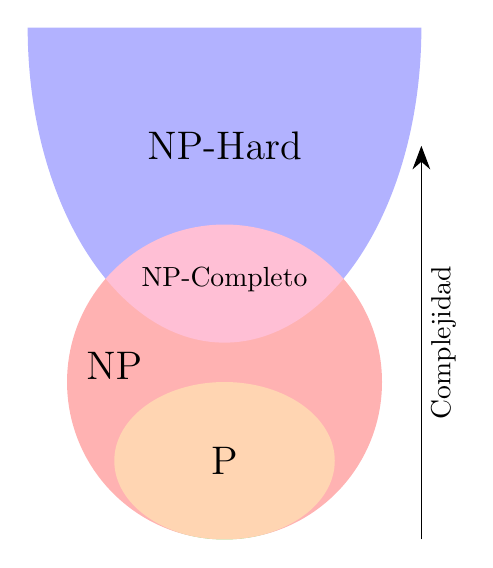
\begin{tikzpicture}
        \usetikzlibrary {arrows.meta}
      \begin{scope}[blend group = soft light]
        \fill[red!30!white]   (90:2) circle (2);
        \fill[green!50!white] (90:1) ellipse (1.4 and 1);
       \fill[blue!30!white] (90:6.5) +(0:2.5cm and 4cm) arc (0:-180:2.5cm and 4cm);
      \end{scope}
      \node at (90:1) [font=\Large] {P};
      \node at (-1.4, 2.2) [font=\Large] {NP};
      \node at (90:5) [font=\Large] {NP-Hard};
      \node at (90:3.3) [] {NP-Completo};
      \draw[-{Stealth[length=3mm]}] (2.5,0)   -- (2.5,5) node[pos=0.5,below,rotate=90] {Complejidad};
    \end{tikzpicture}
    \caption{Diagrama de Venn mostrando la relación entre las clases de complejidad, asumiendo P $\neq$ NP.}
    \label{fig:pnp}
\end{figure}

\section{Cubrimiento por vértices mínimo}
El cubrimiento por vértices mínimo es un problema clásico de la teoría de grafos. A continuación, se enuncian definiciones basadas en el libro~\cite{vertex_cover} que serán útiles en el Capítulo~\ref{ch:tipado}.

\begin{definicion}[Cubrimiento mínimo]\label{def:min_cover}
Un cubrimiento de vértices $C$ para un grafo $G=(V,E)$ es un subconjunto de $V$ tal que para cada arco $uv \in E$ se cumple que $u \in C$ o $v \in C$. Es decir, es un conjunto de vértices $C$ donde cada arco tiene al menos uno de sus extremos en $C$. Tal conjunto se dice que cubre las aristas de $g$. Un cubrimiento mínimo es un cubrimiento con la menor cantidad de vértices.
\end{definicion}

\begin{teorema}\label{teo:cover_lin}
    Sea un grafo $G=(V,E)$. El problema de encontrar el cubrimiento mínimo de vértices $G$ es equivalente a resolver el siguiente problema de $|V|$ incógnitas:
    \begin{mdframed}\begin{align}
        \text{minimizar }&\sum_{v\in V} x_v\label{eq:cov1}\\
        \text{sujeto a }&x_p + x_q \geq 1 \quad \forall pq \in E\label{eq:cov2}\\
        &x_v \in \{0, 1\} \quad \forall v\in V\label{eq:cov3}
    \end{align}\end{mdframed}\qed
\end{teorema}
Este teorema no se va a demostrar, pero se puede entender intuitivamente. A cada vértice se le asigna una variable que por la línea~\ref{eq:cov3} debe ser cero o uno. Si es uno el vértice pertenece al cubrimiento mínimo y si es cero, no. La línea~\ref{eq:cov1} establece que el cubrimiento debe ser el mínimo. La línea~\ref{eq:cov2} se cerciora de que cada arco tenga al menos uno de sus extremos cubiertos.

Por último, aseguramos que la clase de complejidad de este problema es \emph{NP-completo}, es decir que se encuentra en la clase \emph{NP-hard} y a su vez posee una verificación polinomial.

\begin{teorema}
    Encontrar el cubrimiento por vértices mínimo es NP-completo.
\end{teorema}

Este teorema fue probado por primera vez en 1972 por Richard Karp en su famosa publicación ``Reducibility Among Combinatorial Problems''~\cite{cover_np}, donde se prueba que 21 problemas diferentes son NP-completos.

\begin{observacion}
    Lo que es NP-completo es la versión decidible del problema. Es decir aquella que devuelve sí o no. En este caso el problema sería dado un grafo $G=(V,E)$ y un número $k$, responder si existe un cubrimiento de $E$, $S \subseteq V$ tal que $|S|\leq k$. Cabe destacar que si se puede responder esta pregunta en tiempo polinomial, entonces es posible reconstruir el cubrimiento mínimo en tiempo polinomial.
\end{observacion}

\section{El Método Simplex}\label{sec:simplex}

La \emph{programación lineal} es un extenso campo del álgebra lineal dedicado a maximizar o minimizar (optimizar) una función lineal, de tal forma que las variables estén sujetas a una serie de restricciones expresadas mediante un sistema de ecuaciones también lineales. La técnica tradicionalmente usada para resolver problemas de programación lineal es el método Simplex. El mismo se encuentra explicado en el Capítulo 4 de ``Operations Research: Applications and Algorithms''~\cite{simplex}. Este algoritmo resulta útil más adelante en el tipado de $\lambda_\rho$ y se enuncia a continuación.

\begin{definicion}[Método Simplex]\label{def:simplex}
    El algoritmo de Simplex soluciona el problema de maximizar $c^T x$ sujeto a las restricciones $Ax=b$ y $x\geq 0$. Donde $x\in \mathbb{R}^n, c\in \mathbb{R}^n, b\in \mathbb{R}^m, A\in \mathbb{R}^{m\times n}$.
\end{definicion}

No vamos a ahondar en su funcionamiento, pero sí vamos a utilizarlo para resolver la última etapa del tipado.

\section{Funcionalidades de Haskell poco conocidas}

Dado que en este trabajo elegimos Haskell como lenguaje de implementación, discutimos algunos detalles del mismo que resultan relevantes y suelen ser poco comprendidos. Entender estos conceptos es esencial para poder leer el código que se expone en el Capítulo~\ref{ch:implementacion}.

\subsection{Transformadores de Mónadas}
La posibilidad de combinar mónadas resulta atractiva para implementar la traducción presentada en este trabajo, puesto que varios algoritmos necesitan un estado y a su vez tener la posibilidad de producir errores. Si bien podría declararse una mónada que tenga esas dos propiedades, combinar la mónada \texttt{State} y \texttt{Except} es un enfoque más conciso y claro.

Haskell tiene la capacidad de hacer esto empleando los transformadores de mónadas, que son variantes de las mónadas tradicionales. Sus constructores de tipo están parametrizados sobre un constructor de tipo de mónada y producen tipos monádicos combinados~\cite{monads}.

\subsection{Constructores de tipo transformador}
Los constructores de tipos juegan un papel fundamental en el soporte de mónadas de Haskell. En particular, el tipo \texttt{Reader r a} representa  valores de tipo \texttt{a} dentro de una mónada \texttt{Reader} con un entorno de tipo \texttt{r}. El constructor de tipos \texttt{Reader r} es una instancia de la clase \texttt{Monad}, y la función \texttt{runReader::(r->a)} ejecuta una computación en la mónada Reader y devuelve el resultado del tipo \texttt{a}.

Existe una versión transformadora de la mónada Reader, llamada \texttt{ReaderT}, que agrega un constructor de tipo de mónada como parámetro adicional. \texttt{ReaderT r m a} representan los valores de la mónada combinada en la que Reader es la mónada base y \texttt{m} es la mónada interna. \texttt{ReaderT r m} es una instancia de la clase \texttt{Monad}, y la función \texttt{runReaderT::(r -> m a)} realiza un cálculo en la mónada combinada y devuelve un resultado de tipo \texttt{m a}.

Utilizando las versiones transformadoras de las mónadas, podemos producir mónadas combinadas de forma muy sencilla. \texttt{ReaderT r IO} es una mónada combinada de Reader+IO. También podemos generar la versión sin transformador de una mónada a partir de la versión transformadora aplicándola a la mónada de identidad. Entonces \texttt{ReaderT r Identity} es la misma mónada que \texttt{Reader r}.

\subsection{Lifting}

Cuando usamos mónadas combinadas creadas por los transformadores de mónadas, evitamos tener que administrar explícitamente los tipos de mónadas internas, lo que da como resultado un código más claro y simple. En lugar de escribir código adicional dentro de las implementaciones para manipular valores del tipo de la mónada interna, podemos recurrir a las operaciones de lifting para traer funciones de la mónada interna a la mónada combinada. Esto quiere decir que sabiendo como manipular cada mónada involucrada es posible escribir código que opere sobre ambas mónadas.

La familia de funciones \texttt{liftM} se utilizan para elevar funciones no monádicas a una mónada. Cada transformador de mónada proporciona una función de elevación que se emplea para elevar un cálculo monádico a una mónada combinada. Los transformadores también proporcionan una función \texttt{liftIO}, que es una versión de lift que está optimizada para hacer lifting de la mónada IO.

\section{\texorpdfstring{$\lambda_\rho$, un cálculo lambda con matrices de densidad}{Lambda Rho, un cálculo lambda con matrices de densidad}}\label{sec:lamrho_classic}

En 2017 Díaz-Caro presenta $\lambda_\rho$~\cite{lamrho}, un cálculo lambda cuántico que usa matrices de densidad para representar estados cuánticos. El mismo se caracteriza por codificar los estados directamente sobre los términos, a diferencia de otros lenguajes como el descrito por Selinger~\cite{SelingerMSCS04} que recurre a las matrices de densidad únicamente para su interpretación. Esto genera lenguajes más simples, ya que no se necesita una clausura para hacer referencia el estado cuántico.
 
El cálculo $\lambda_\rho$ utiliza un sistema de reducción probabilístico para modelar la operación de medición. Es importante resaltar que, si bien podemos codificar estados mixtos, la medición probabilística va a generar un estado puro. En las siguientes secciones se detalla la definición, el tipado y las reglas de reducción del lenguaje.

%%%%%==== Subsección ====%%%%%%
\subsection{\texorpdfstring{Definición de $\lambda_\rho$}{Definición de Lambda Rho}}

Se puede entender a $\lambda_\rho$ como una extensión del lambda cálculo simplemente tipado con términos que representan los cuatro postulados cuánticos y un término ($\textsf{letcase}$) para el control clásico basado en el resultado de las mediciones. Siguiendo esta idea se define el conjunto de términos de $\lambda_\rho$ ($\Lambda_\rho$) en la Definición \ref{lambda_rho_def}.



% \needspace{8\baselineskip}
\begin{definicion}[Gramática de $\lambda_\rho$]
\label{lambda_rho_def}
\begin{align*}
t ::= &\;x \mid \lambda x.t \mid t\;t \tag{Lambda cálculo estándar}\\
 \mid&\; \rho^n \mid U^n t \mid \pi^m t \mid t \otimes t \tag{Postulados cuánticos}\\
 \mid&\; (b^m, \rho^n) \mid \textsf{letcase }x = t \textsf{ in } \{t,\dots,t\} \tag{Control clásico}
\end{align*}
donde:
\begin{itemize}
    \item
    \item $n,m \in \mathbb{N}, m \leq n$.
    \item $\rho^n$ es una matriz de densidad de n-qubits, es decir, una matriz positiva de $2^n \times 2^n$ con traza 1.
    \item $b^m \in \mathbb{N}_0, 0 \leq b^m < 2^m$.
    \item ${t,\dots,t}$ contiene $2^m$ términos
    \item $U^n$ es un operador unitario de dimensión $2^n \times 2^n$, es decir, una matriz $2^n \times 2^n$ tal que $(U^n)^\dagger = (U^n)^{-1}$.
    \item $\pi^n=\{\pi_0,\dots,\pi_{2^n-1}\}$, describe una medición cuántica en la base computacional, donde cada $\pi_i$ es un operador proyector de dimensión $2^n$ que proyecta a un vector de la base canónica.
\end{itemize}
\end{definicion}


\subsection{\texorpdfstring{Tipado de $\lambda_\rho$}{Tipado de Lambda Rho}}
El sistema de tipos de $\lambda_\rho$ es afín, por lo que las variables pueden ser usadas a lo sumo una sola vez. Otra característica peculiar es que contiene enteros. Por ejemplo, el tipo `3' representa un estado cuántico de 3 qubits. Mientras que el tipo `$(3, 5)$' es el resultado de una medición de 3 qubits sobre un estado de 5 qubits. Sobre estos valores se agregan las funciones de alto orden del cálculo lambda afín.

Para formalizar el tipado introducimos contextos que son un mapeo entre variables y sus tipos. Por ejemplo $\Delta = x:A$ es un contexto que le asigna el tipo $A$ a la variable $x$. Dados dos contextos $\Delta$ y $\Gamma$, denotamos \emph{$\Delta,\Gamma$} como la unión de ambos contextos:
\[
(\Delta,\Gamma)(x) = \begin{cases}
    \Delta(x) \text{ si } x\in\mathrm{dom}(\Delta) \\
    \Gamma(x) \text{ si } x\in\mathrm{dom}(\Gamma)
\end{cases}
\]

\begin{definicion}[Tipado de $\lambda_\rho$]
\label{def:tipado_lambda}

Siendo $n,m \in \mathbb{N}, m\leq n$,
\begin{align*}
A := n \mid (m, n) \mid A \multimap A
\end{align*}
 \[\arraycolsep=5pt\def\arraystretch{2.6}
   \begin{array}{ccc}
     \infer[\mathtt{ax}]
     {\Gamma, x : A \vdash x : A}
     {}
     &
         \infer[\multimap_i]
         {\Gamma \vdash \lambda x.t : A \multimap B}
         {\Gamma, x : A \vdash t : B}
     &
         \infer[\multimap_e]
         {\Gamma, \Delta \vdash t\;r : B}
         {\Gamma \vdash t : A \multimap B \quad \Delta \vdash r : A}
   \end{array}
 \]
 \[\arraycolsep=5pt\def\arraystretch{2.6}
   \begin{array}{ccc}
     \infer[\mathtt{ax}_\rho]
     {\Gamma \vdash \rho^n : n}
     {}
     &
         \infer[\mathtt{u}]
         {\Gamma \vdash U^m\;t : n}
         {\Gamma \vdash t : n}
     &
         \infer[\pi]
         {\Gamma \vdash \pi^m t : (m, n)}
         {\Gamma \vdash t : n}
   \end{array} 
 \]
 \[\arraycolsep=5pt\def\arraystretch{2.6}
   \begin{array}{cc}
     \infer[\otimes]
     {\Gamma, \Delta \vdash t \otimes r : n + m}
     {\Gamma \vdash t: n \quad \Delta \vdash r : m}
     &
         \infer[\mathtt{ax_{am}}]
         {\Gamma \vdash (b^m, \rho^n) : (m, n)}
         {}
   \end{array}
 \]
 \[\arraycolsep=5pt\def\arraystretch{2.6}
   \begin{array}{c}
     \infer[\mathtt{lc}]
     {\Gamma \vdash \textsf{letcase } x = r \textsf{ in  }\{t_0,\dots,t_{2^m-1}\} : A}
     {x:n\vdash t_0 : A \quad \dots\quad x:n\vdash t_{2^m-1}:A\quad \Gamma \vdash r:(m, n)}
   \end{array}
 \]

\end{definicion}

\subsection{Reglas de reducción}
Las reglas de reducción dadas en la Definición~\ref{def:reduccion_lambda1}, son descritas por la relación $\redlam_p$, que es una relación probabilística donde $p$ es la probabilidad de que tal reducción ocurra.


Si $U^m$ es aplicado a $\rho^n$, con $m \leq n$, definimos $\overline{U ^m} = U^m \otimes I^{n-m}$. Similarmente, cuando $\pi^m$ es aplicado a $\rho^n$, con $m \leq n$, definimos $\overline{\pi^m}$ como el conjunto de operadores de medición $\{\pi_0\otimes I^{n-m}, \dots, \pi_{2^m-1} \otimes I^{n-m}\}$. 

Antes de dar las reglas es conveniente dejar en claro la notación para las sustituciones.


\subsubsection{Sustitución de expresiones}

La sustitución se define de la forma usual. Escribimos $A$ en lugar de $\alpha$ como $[A/\alpha]$ y la sustitución nula como $[-]$. Aplicar la sustitución $\sigma$ a la expresión $E$ se denota $\sigma E$.
Las sustituciones $\sigma$ y $\mu$ se dice que son iguales si y solo sí $\forall x\;\sigma(x)=\mu(x)$.
Al ser funciones, las sustituciones pueden ser compuestas y aplicadas. El dominio y rango de una sustitución se definen de la siguiente manera:
\begin{align}
    \text{dom}(\sigma) &= \{\alpha / \alpha \neq \sigma(\alpha)\} \\
    \text{rng}(\sigma) &= \{\sigma(\alpha) / \alpha \in \text{dom}(\sigma)\} 
\end{align}

Estas definiciones permiten probar que $\sigma=\sigma' \implies \text{dom}(\sigma) = \text{dom}(\sigma')$ y $\text{rng}(\sigma)=\text{rng}(\sigma')$.


Finalmente, se enuncian las reglas de reducción de $\lambda_\rho$.
\begin{figure}[H]
\begin{definicion}[Reglas de reducción de $\lambda_\rho$]
\label{def:reduccion_lambda1}
\begin{align*}
(\lambda x.t)\;r &\redlam_1 [r/x]t\\
U^m\;\rho^n &\redlam_1 {\rho'}^n \qquad \text{ con } {\rho'}^n = \overline{U^m}\;\rho^n\;\adj{\overline{U^m}} \\
\pi^m\;\rho^n &\redlam_{p_i} (i^m, \rho_i^n) \;\, \text{ con }
\begin{cases}
p_i = \tr(\adj{\overline{\pi^m_i}}\;\overline{\pi^m_i}\;\rho^n)\\
\rho^n_i = (\overline{\pi^m_i}\;\rho^n\;\adj{\overline{\pi^m_i}})/p_i
\end{cases}\\
\rho \otimes \rho' &\redlam_1 \rho'' \qquad \text{ con } \rho'' = \rho \otimes \rho' \\
\textsf{letcase } x = (b^m, \rho^n) &\textsf{ in } \{t_0, \dots, t_{2^m-1}\} \redlam_1 [\rho^n/x] t_{b^m}
\end{align*}
 \[\arraycolsep=10pt\def\arraystretch{2.6}
   \begin{array}{cccc}
     \infer
     {\lambda x.t \redlam_p \lambda x.r}
     {t \redlam_p r}
     &
         \infer
         {t\;s\redlam_p r\;s}
         {t \redlam_p r}
     &
         \infer
         {s\;t\redlam_p s\;r}
         {t \redlam_p r}
     &
         \infer
         {U^m\;t\redlam_p U^m\;r}
         {t \redlam_p r}
   \end{array}
 \]
 \[\arraycolsep=10pt\def\arraystretch{2.6}
   \begin{array}{cccc}
     \infer
     {\pi^n\;t \redlam_p \pi^n\;r}
     {t \redlam_p r}
     &
         \infer
         {t\otimes s \redlam_p r \otimes s}
         {t \redlam_p r}
     &
         \infer
         {s\otimes t \redlam_p s \otimes r}
         {t \redlam_p r}
   \end{array} 
 \]
 \[\arraycolsep=10pt\def\arraystretch{2.6}
   \begin{array}{c}
     \infer
     {\textsf{letcase }x = t \textrm{ in } \{s_0,\dots,s_n\} \redlam_p \textsf{letcase }x = r \textrm{ in } \{s_0,\dots,s_n\} }
     {t \redlam_p r}
   \end{array}
 \]
\end{definicion}
\end{figure}

La siguiente notación es útil para cuando queremos hacer varios pasos de la reducción de forma sucesiva.

\begin{figure}[H]
\begin{definicion}[$\rightarrow_p^*$]
Para cualquier relación probabilística $\rightarrow_p$, denotamos $\rightarrow_p^*$ a su cierre reflexivo y transitivo. Es decir:
 \[\arraycolsep=10pt\def\arraystretch{2.6}
   \begin{array}{cc}
    \infer
     {x \rightarrow_1^* x}
     {}
     &
     \infer
     {x \rightarrow_{pq}^* z}
     {x \rightarrow_p^* y \quad y \rightarrow_q z}
   \end{array}
 \]
\end{definicion}
\end{figure}

% {enunciar teoremas de correctitud: SR, SN, confluencia y eq con SV06}?

% Reducción de Sujeto (Subject Reduction): La Reducción de Sujeto es una propiedad en la teoría de tipos y la semántica formal de lenguajes de programación que establece que si una expresión en un lenguaje de programación está bien tipada, entonces, cuando se realiza una reducción o evaluación de la expresión, la expresión resultante seguirá estando bien tipada según las reglas del sistema de tipos del lenguaje. En otras palabras, asegura que la información de tipo se conserva durante la evaluación, lo que es fundamental para garantizar la seguridad de tipos y la corrección en los programas escritos en ese lenguaje. La Reducción de Sujeto es una propiedad esencial en la verificación formal y la teoría de lenguajes de programación.

% SN (Normalization): "SN" stands for "Strong Normalization" or "Strong Normalization Property." It is related to termination but is more specific. SN is a property used to show that a program or system reduces or simplifies its computations and expressions in such a way that it always reaches a normal form, meaning there are no more reduction steps possible. In other words, SN ensures that computations terminate and produce results while also ensuring that the results are in a simplified or normalized state.
% \begin{teorema}[SR: Reducción de términos de $\lambda_\rho$]
%     $\lambda_\rho$ es fuertemente reducible. Es decir que cualquier expresión eventualmente termina en una expresión normal. \qed
% \end{teorema}
% \begin{teorema}[SN: Normalización fuerte de $\lambda_\rho$]
%     $\lambda_\rho$ es fuertemente normalizado. Es decir,  \qed
% \end{teorema}


% \section{Interpretación}